%%test.tex
%\documentclass{article}
%%\usepackage{CJKutf8}
%\usepackage{xeCJK}
%\usepackage{amsmath}
%\usepackage{colortbl}
%\usepackage{graphicx}
%%\begin{CJK}{UTF8}{gbsn}
%%\end{CJK}
%\end{document}
\documentclass{article}
\usepackage{color}
\usepackage{amsmath}
\usepackage{hyperref}
\usepackage[UTF8]{ctex}
\usepackage{graphicx}
\usepackage{xeCJK}
\usepackage{listings}
\lstset{                        %Settings for listings package.
	language=[ANSI]{C},
	basicstyle=\footnotesize,
	breakatwhitespace=false,
	breaklines=true,
	captionpos=b,
	extendedchars=false,
	% frame=single,%shadowbox
	framerule=0pt,
	morekeywords={*,define,*,include...},
	numbersep=5pt,
	showspaces=false,
	showstringspaces=false,
	showtabs=false,
	stepnumber=2,
	tabsize=4,
	title=\lstname
}

\begin{document}
\title{课程实验}
\author{师清}
\maketitle
\section{cuda编程模型}
\subsection{异构并行计算}
\noindent
\textcolor{blue}{CPU+GPU}\\
CPU:heavy-weight,for complex control logic\\
GPU:light-weight,for data-parallel tasks with simple control logic\\
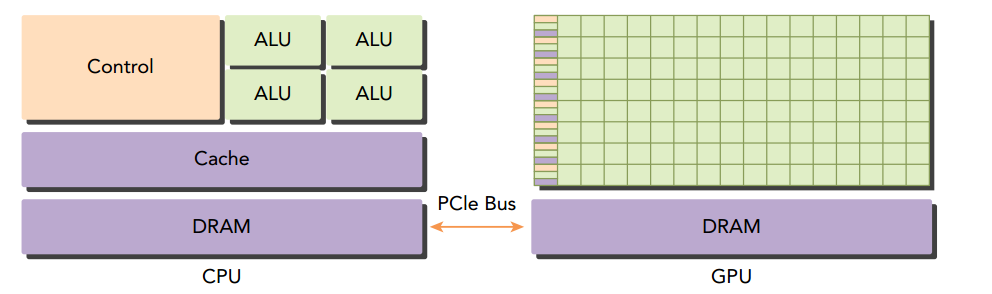
\includegraphics[width=0.9\textwidth]{assets/cpu_gpu.png}\\
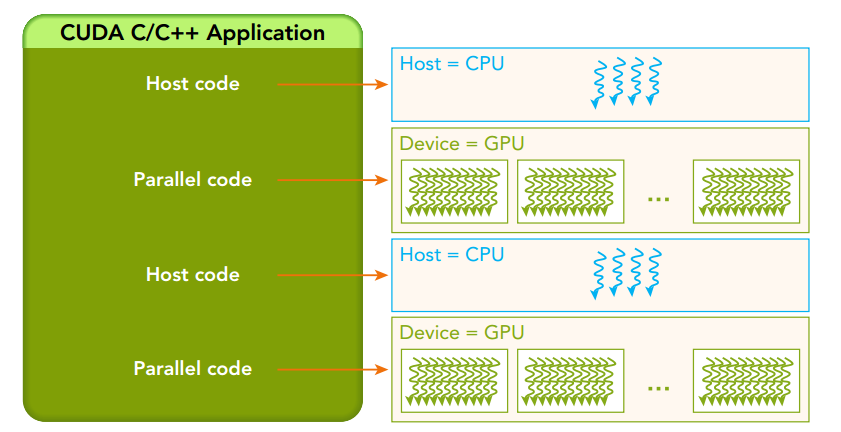
\includegraphics[width=0.9\textwidth]{assets/cuda.png}\\
Peak computational performance:TFLOPS(每秒万亿次的浮点运算)\\
Memory bandwidth:GB/s\\
\subsection{cuda编程架构}
\noindent
\underline{CUDA: A Platform for Heterogeneous Computing}\\
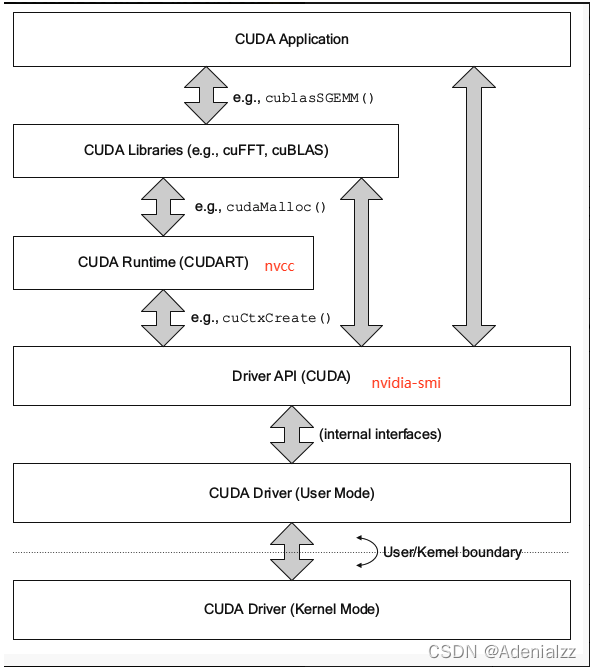
\includegraphics[width=0.9\textwidth]{assets/cuda-platform.png}\\
两种api:CUDA Driver API 和 CUDA Runtime API\\
\subsubsection{物理上}
\noindent
nvidia gpu架构的演变:\\
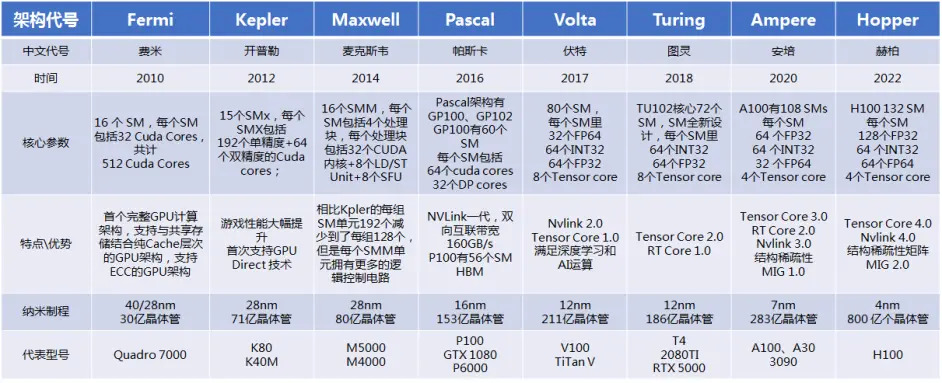
\includegraphics[width=0.9\textwidth]{assets/gpu.jpg}\\
Fermi架构:第一个完整的GPU计算架构\footnote{\href{https://www.nvidia.com/content/PDF/fermi_white_papers/NVIDIA_Fermi_Compute_Architecture_Whitepaper.pdf}{Fermi架构}}:\\
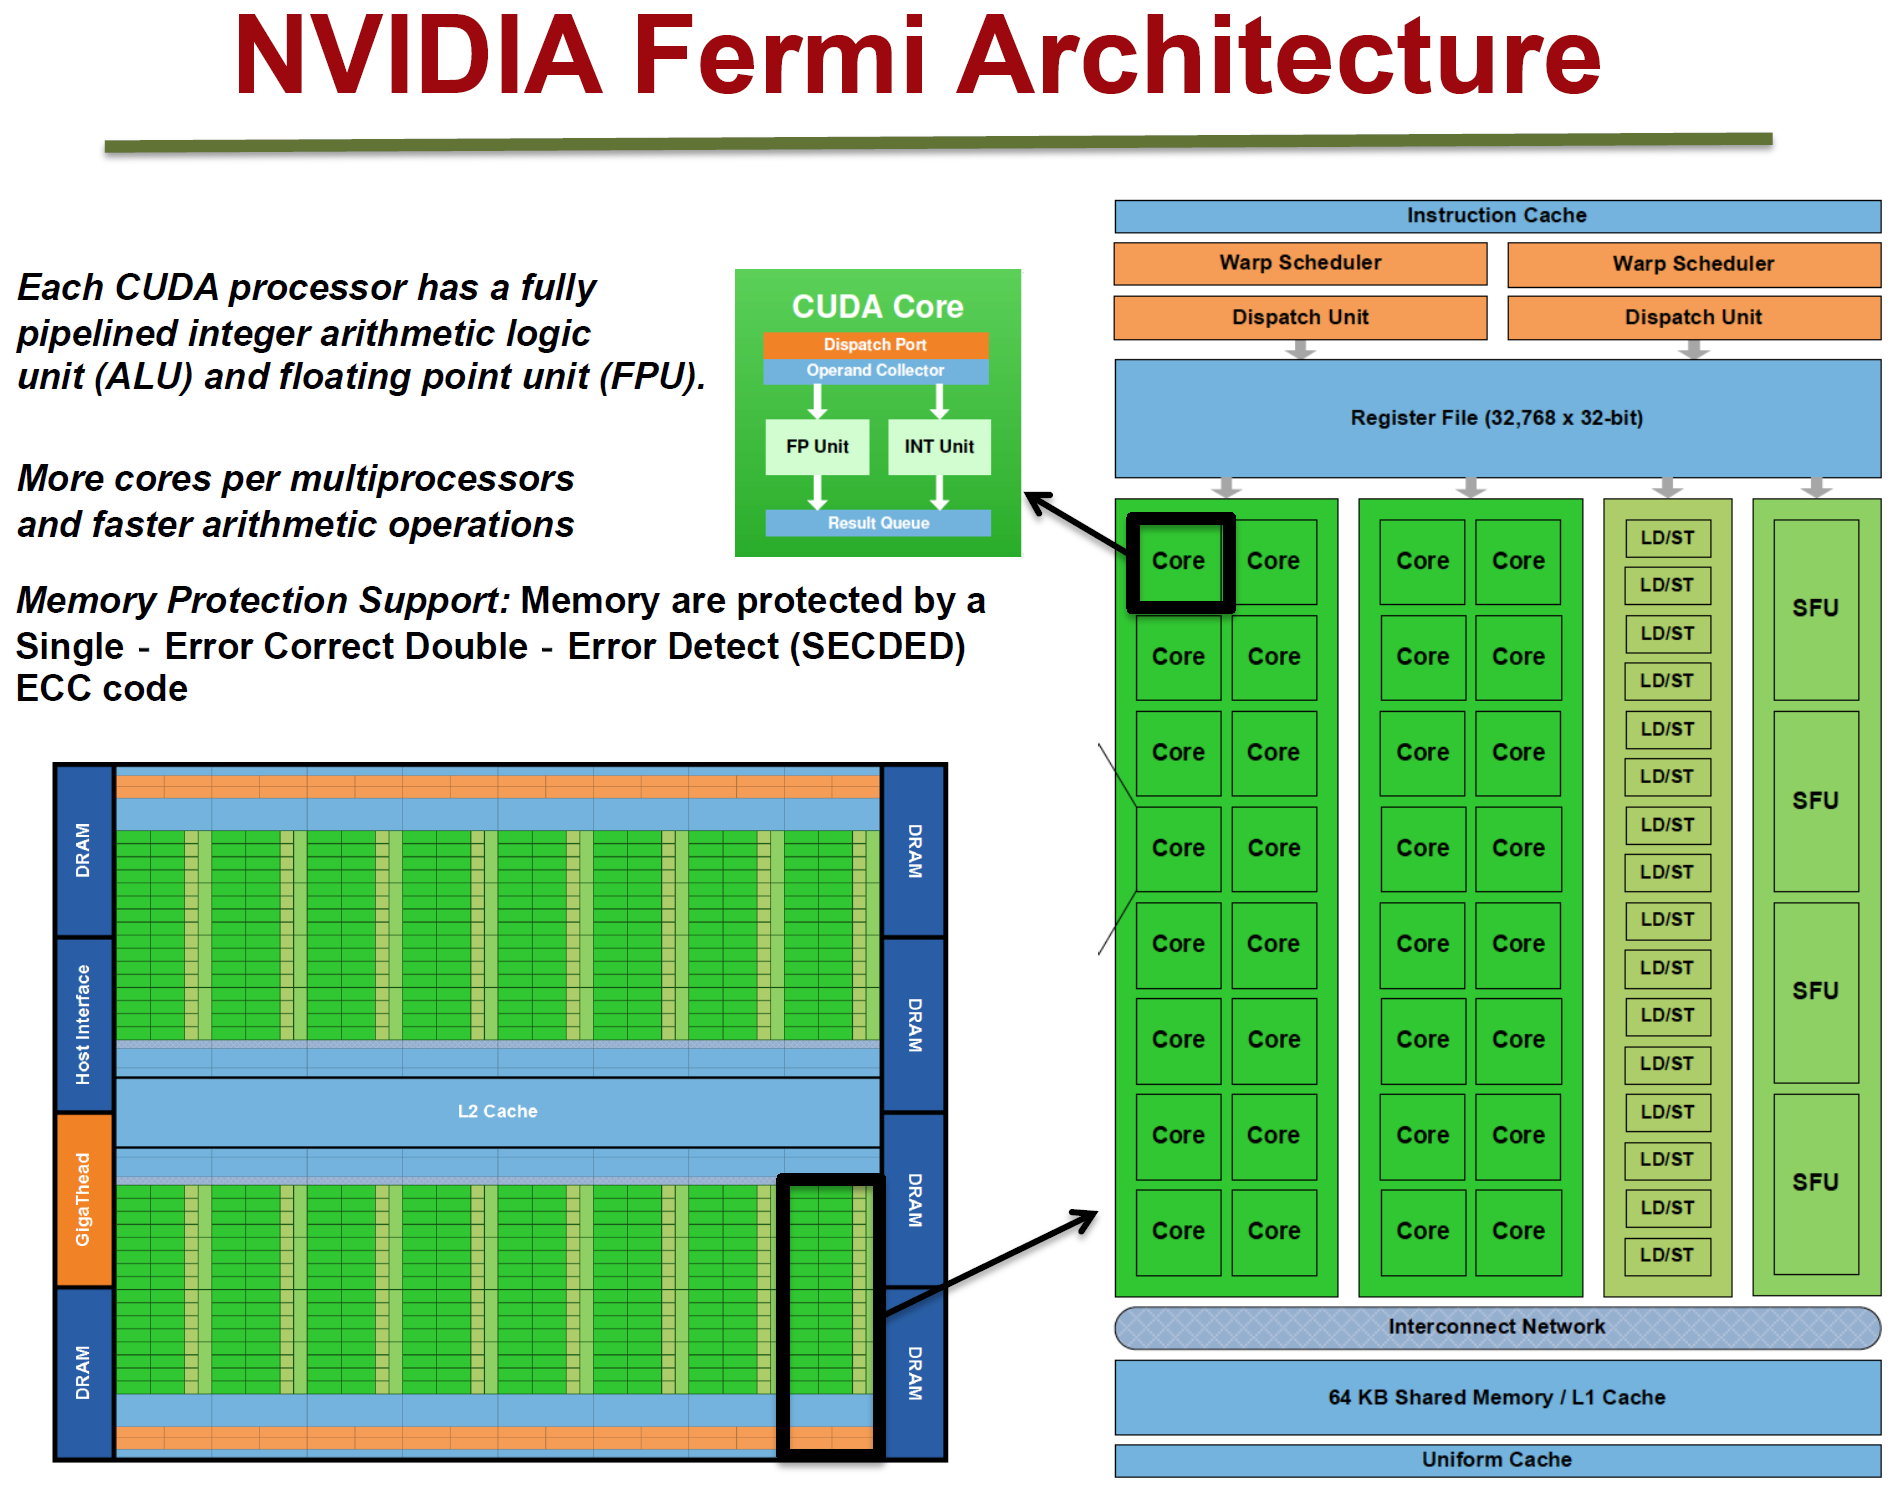
\includegraphics[width=0.9\textwidth]{assets/fermi.png}\\
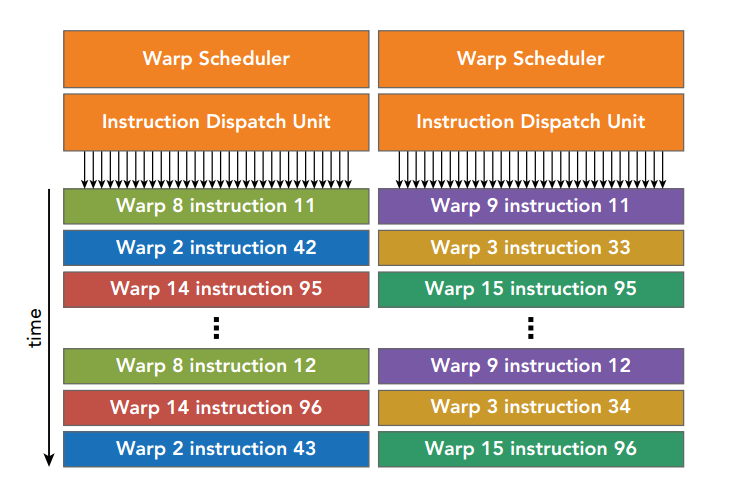
\includegraphics[width=0.9\textwidth]{assets/warp.png}\\
单个SM(Stream Multiprocessor)包括如下组成部分:
\begin{itemize}
	\item Core,也叫流处理器Stream Processor
	\item LD/ST(load/store)模块来加载和存储数据
	\item SFU(Special function units)执行特殊数学运算(sin、cos、log等
	\item 寄存器(Register File)
	\item L1缓存
	\item 全局内存缓存(Uniform Cache)
	\item 纹理缓存(Texture Cache)
\end{itemize}

\subsubsection{逻辑上}
\noindent
\textcolor{blue}{thread hierarchy}\footnote{\href{https://blog.csdn.net/yangjinyi1314/article/details/124905292}{cuda核函数的并行机制}}:\\
grid,block,thread,warp\\
gridDim(blockIdx.x
blockIdx.y,
blockIdx.z),blockDim(threadIdx.x,threadIdx.y,threadIdx.z)\\

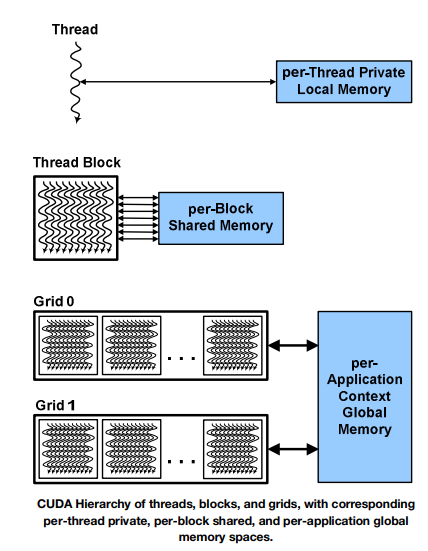
\includegraphics[width=0.9\textwidth]{assets/thread.png}\\
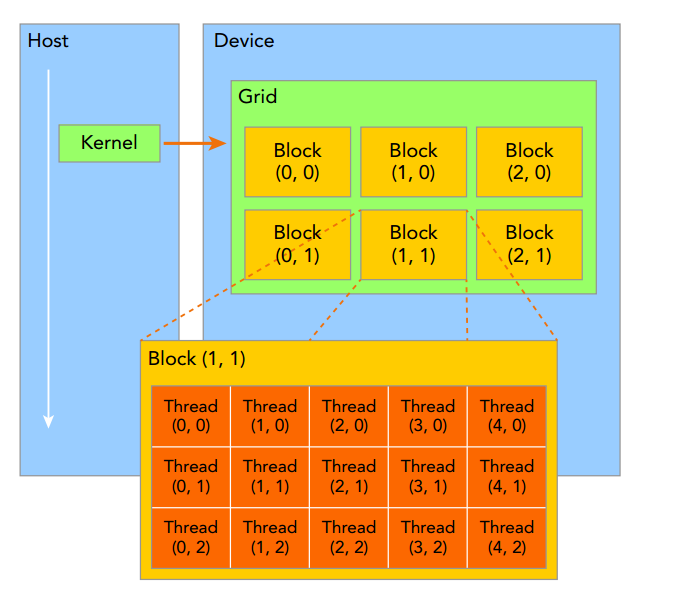
\includegraphics[width=0.9\textwidth]{assets/thread2.png}\\
\textcolor{blue}{memory hierarchy}\footnote{\href{https://blog.csdn.net/xukang95/article/details/102855750}{cuda内存层次}}:\\
register,local memory,shared memory,constant memory,texture memory,global memory,host memory\\
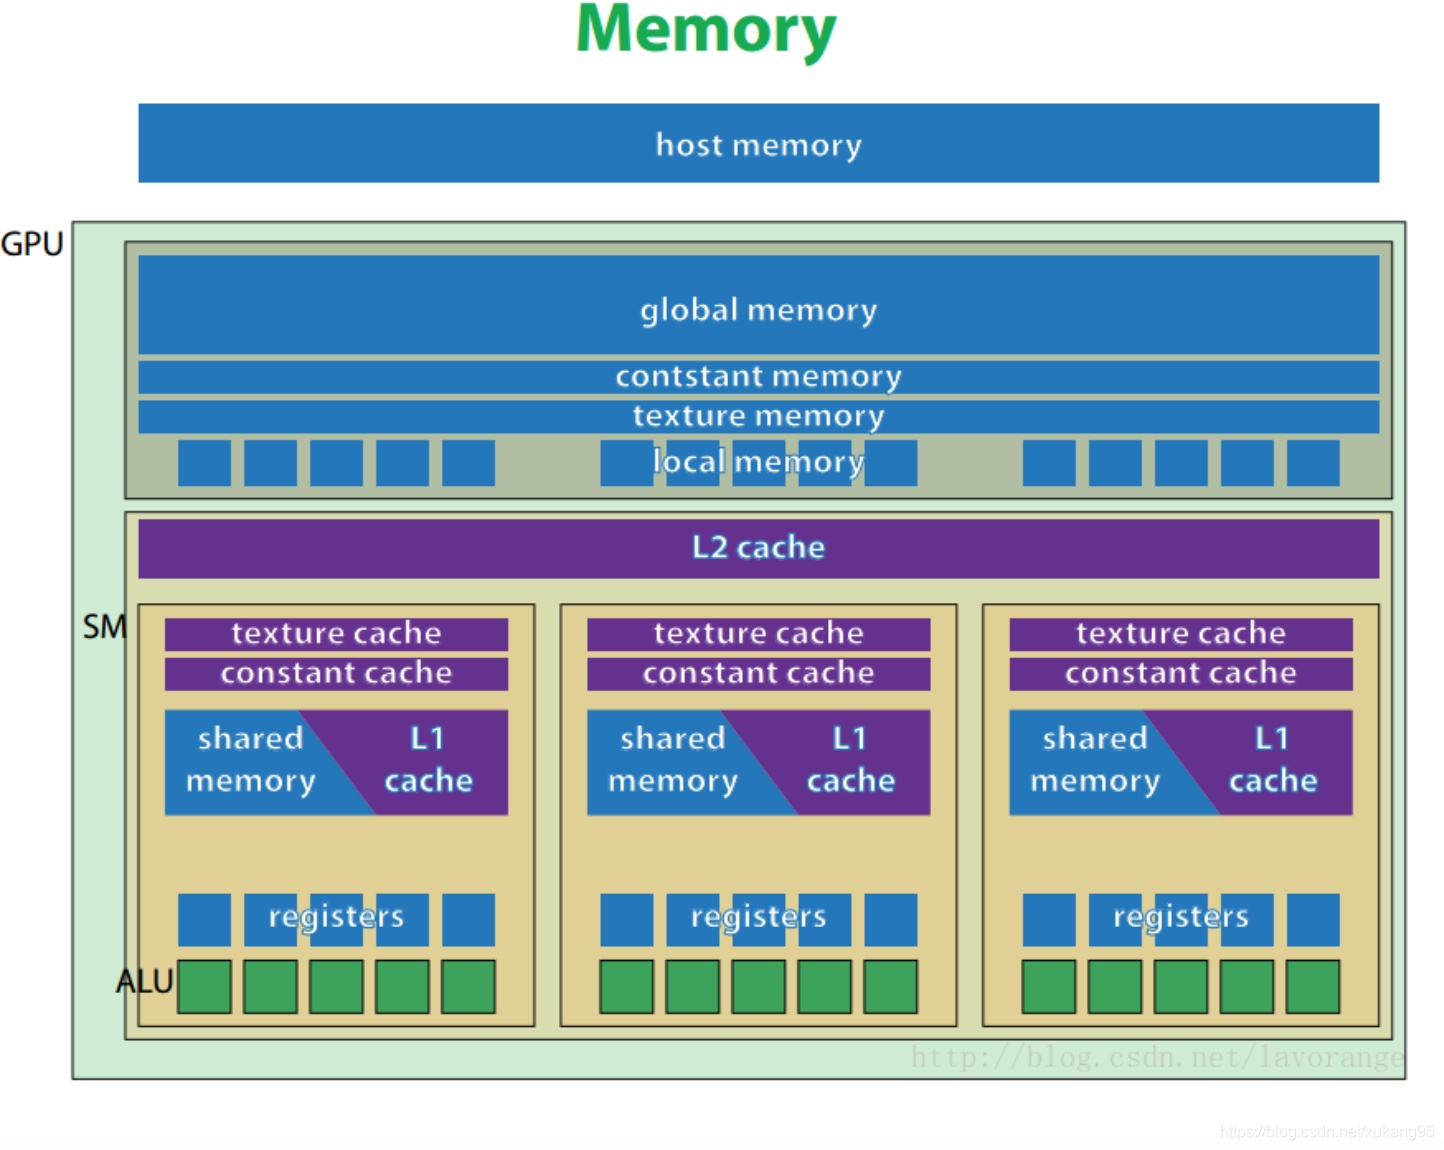
\includegraphics[width=0.9\textwidth]{assets/mem.jpg}\\

\subsubsection{CUDA C}
\noindent

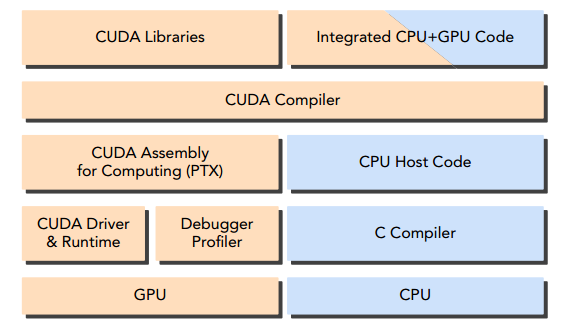
\includegraphics[width=0.9\textwidth]{assets/cudac.png}\\
\textcolor{blue}{nvcc},编译工具\footnote{\href{https://docs.nvidia.com/cuda/cuda-compiler-driver-nvcc/index.html}{nvcc编译过程}}\\
nvprof已被弃用,使用下面两个作为profile工具\\
\textcolor{blue}{NVIDIA Nsight Compute},ncu  \\
\textcolor{blue}{NVIDIA Nsight Systems},nsys\\
CUDA C syntax
\subsection{本机实验环境}
\noindent
GPU:NVIDIA GeForce RTX 3050 Laptop GPU\\
Driver Version: 470.141.03   \\
CUDA Version: 11.4\\
nvcc:release 11.0, V11.0.194

\section{cuda编程练习}
\noindent
(APOD开发模型,即:Assess, Parallelize, Optimize, Deploy)\\
\underline{\href{https://github.com/buyizhiyou/cuda-tutorial}{\textcolor{blue}{代码地址}}}





\subsection{矩阵加法}
\subsubsection{代码}
\begin{lstlisting}
#include <cuda_runtime.h>
#include <stdio.h>
#include "../include/myhelp.h"

void sumArrays(float* a,float* b,float* res,const int size){
	for(int i=0;i<size;i++){
		res[i]=a[i]+b[i];
	}
}

__global__ void sumArraysGPU(float* a,float* b,float* res){
	int i=threadIdx.x;
	res[i]=a[i]+b[i];
}

int main(int argc,char** argv){
	int dev=0;
	cudaSetDevice(dev);
	
	int n=32;
	printf("Vector size:%d\n",n);
	int nByte=sizeof(float)*n;
	float* a_h=(float*)malloc(nByte);
	float* b_h=(float*)malloc(nByte);
	float* res_h=(float*)malloc(nByte);
	float* res_from_gpu_h=(float*)malloc(nByte);
	memset(res_h,0,nByte);
	memset(res_from_gpu_h,0,nByte);
	
	float* a_d,* b_d,* res_d;
	CHECK(cudaMalloc((float**)&a_d,nByte));
	CHECK(cudaMalloc((float**)&b_d,nByte));
	CHECK(cudaMalloc((float**)&res_d,nByte));
	
	initialData(a_h,n);
	initialData(b_h,n);
	
	CHECK(cudaMemcpy(a_d,a_h,nByte,cudaMemcpyHostToDevice));
	CHECK(cudaMemcpy(b_d,b_h,nByte,cudaMemcpyHostToDevice));
	
	dim3 block(n);
	dim3 grid(n/block.x);
	sumArraysGPU<<<grid,block>>>(a_d,b_d,res_d);
	printf("Execution configuration<<<%d,%d>>>",block.x,grid.x);

	CHECK(cudaMemcpy(res_from_gpu_h,res_d,nByte,cudaMemcpyDeviceToHost));
	sumArrays(a_h,b_h,res_h,n);
	
	checkResult(res_h,res_from_gpu_h,n);
	cudaFree(a_d);
	cudaFree(b_d);
	cudaFree(res_d);
	
	free(a_h);
	free(b_h);
	free(res_h);
	free(res_from_gpu_h);
	
	return  0;
}


\end{lstlisting}

\subsubsection{实验结果}
\noindent
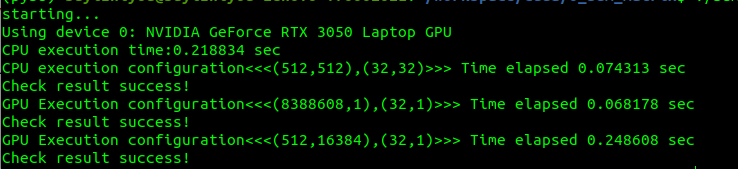
\includegraphics[width=0.9\textwidth]{assets/matrix.png}
\subsubsection{分析总结}
\noindent
不同的execution configuration会影响执行性能,因此尝试不同的grid和block dimensions可能产生更好的性能。

\subsection{warp divergence}
\subsubsection{实验结果}
\noindent
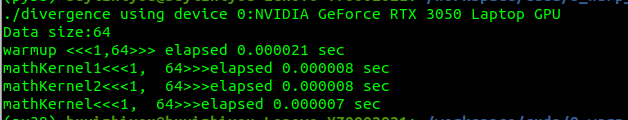
\includegraphics[width=0.9\textwidth]{assets/warp_d.png}
\subsubsection{分析总结}
\noindent
同一个warp内的线程必须执行同一条指令,当线程内存在控制流时,不同线程可能有不同的执行路径,这会降低核函数效率,所以要尽量避免同一个warp内的线程分化。

\subsection{数组求和}
\subsubsection{实验结果}
\noindent
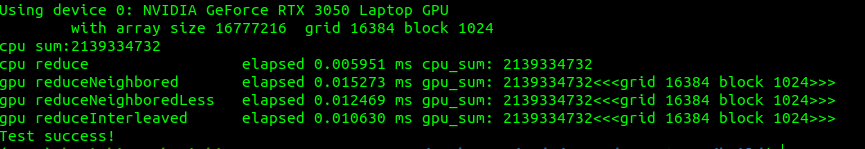
\includegraphics[width=0.9\textwidth]{assets/sum.png}
\subsubsection{分析总结}
\noindent
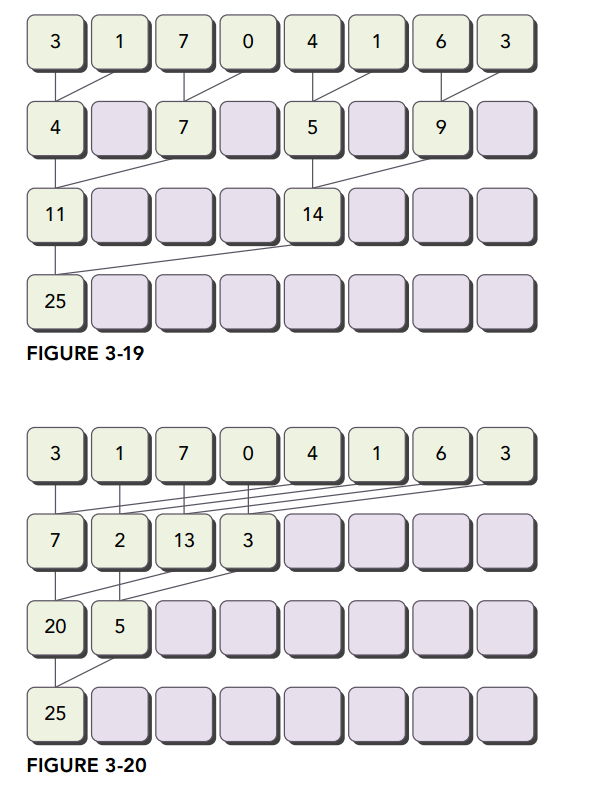
\includegraphics[width=0.9\textwidth]{assets/interleave.png}
\begin{itemize}
	\item The Parallel Reduction Problem(并行规约问题),避免分支分化(branch divergence)
	\item 使用interleaved pair approach替代neighbored approach,性能提升
	\item Synchronization:system-level 和 block-level,分别使用cudaDeviceSynchronize()和\_syncthreads()
\end{itemize}


\subsection{循环展开}
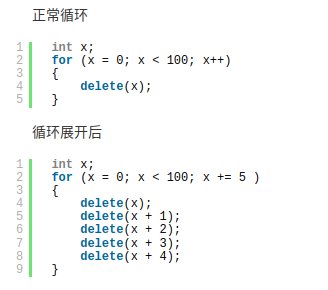
\includegraphics[width=0.5\textwidth]{assets/unroll.png}
\subsubsection{实验结果}
\noindent
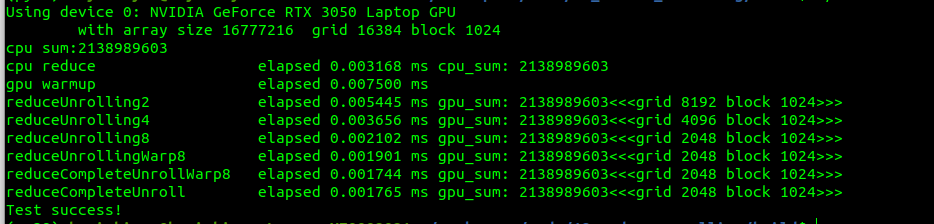
\includegraphics[width=0.9\textwidth]{assets/loop.png}
\subsubsection{分析总结}
\noindent
\begin{itemize}
	\item 循环展开是一种通过减少分支和循环指令来优化程序性能的方法,利用手动重复执行某个操作来代替一个循环体
	\item 循环展开为什么能提升性能?编译器可以进行low-level的指令优化(指令流水的充分调度)
\end{itemize}


\subsection{结构体数组vs数组结构体}
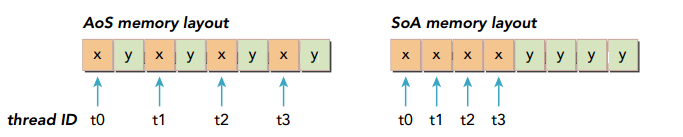
\includegraphics[width=0.9\textwidth]{assets/sc.png}
\subsubsection{实验结果}
\noindent
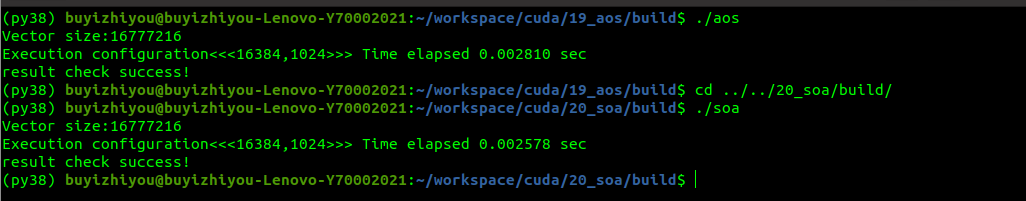
\includegraphics[width=0.9\textwidth]{assets/aos.png}
\subsubsection{分析总结}
\noindent
\begin{itemize}
	\item 内存访问模式:理想的是对齐联合访问(aligned and coalesced access pattern)
	\item 并行编程范式,尤其是SIMD(单指令多数据)对SoA更友好。CUDA中普遍倾向于SoA因为这种内存访问可以有效地合并。
\end{itemize}


\subsection{矩阵转置}
\subsubsection{实验结果}
\noindent
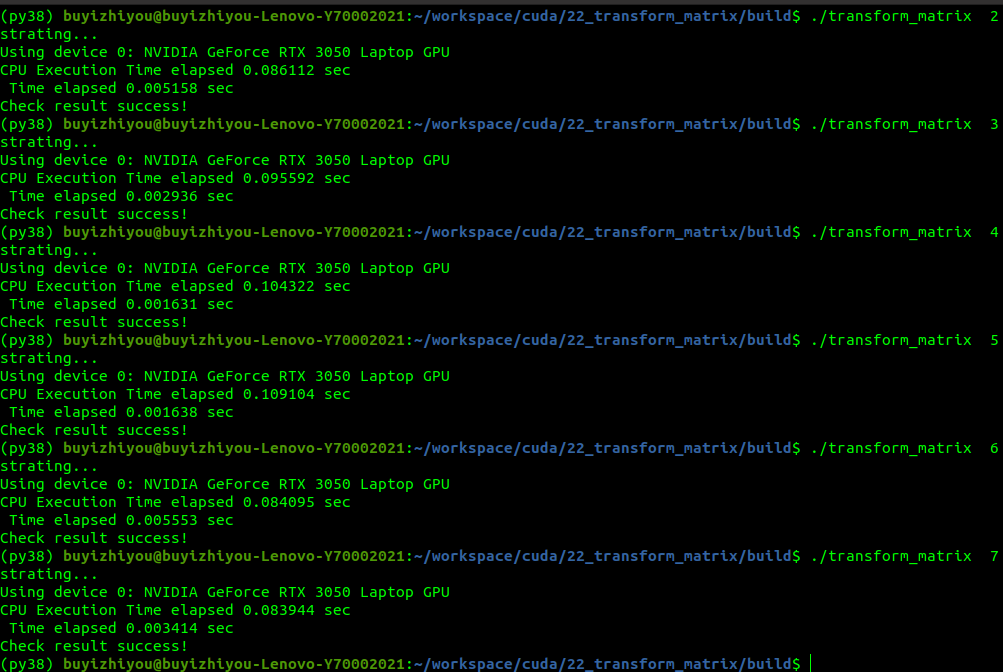
\includegraphics[width=0.9\textwidth]{assets/diag.png}
\subsubsection{分析总结}
\noindent
\begin{itemize}
	\item 当分析一个核函数性能时,注意分析memory latency(memory bandwidth),一个良好的内存访问模式能提高存储带宽
	\item 2,3分别是按行读取和按列读取,按列读取的吞吐量大于按行读取的原因是缓存命中
	\item 4,5分别是利用循环展开提升性能
	\item 6,7是使用对角化的方式,提高对存储块的均匀访问
\end{itemize}


\subsection{共享内存的读写}
memory bank:\\
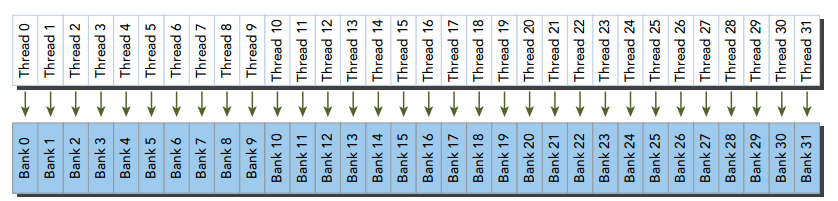
\includegraphics[width=0.9\textwidth]{assets/bank.png}\\

padding:\\
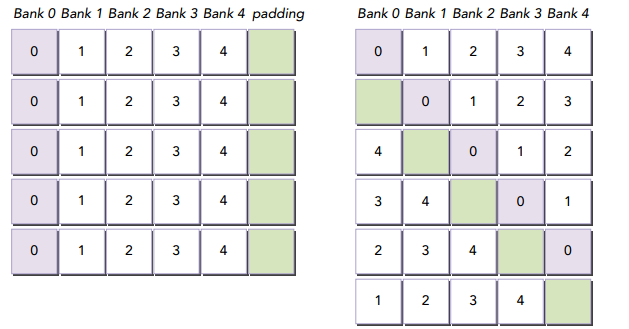
\includegraphics[width=0.9\textwidth]{assets/padding.png}
\subsubsection{实验结果}
\noindent
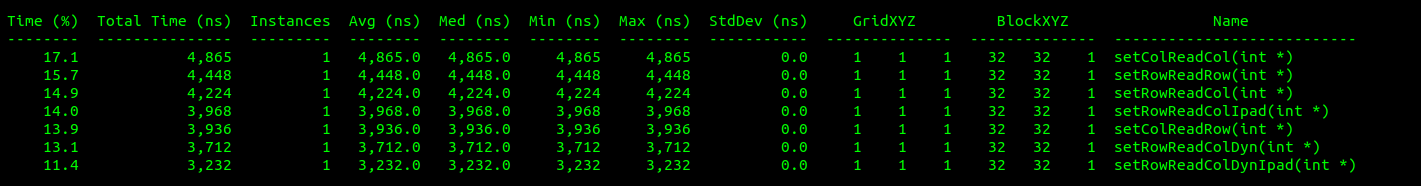
\includegraphics[width=0.9\textwidth]{assets/sm.png}
\subsubsection{分析总结}
\noindent
\begin{itemize}
	\item shared memory的行主序读写和列主序读写,按照行主序读和写,减少共享内存冲突(bank conflict)
	\item shared memory的动态分配,在$kernel\_name<<<...>>>$里面可以指定分配的shared memory
	\item shared memory的padding,减少back conflicts
\end{itemize}

\subsection{利用共享内存做reduce求和任务}
\subsubsection{实验结果}
\noindent
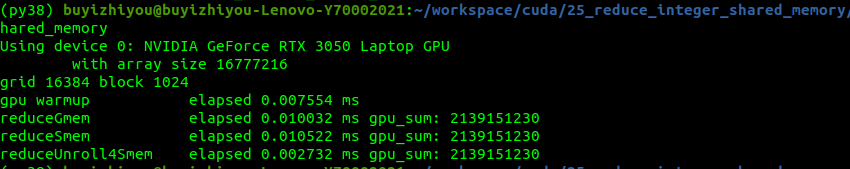
\includegraphics[width=0.9\textwidth]{assets/smem.png}
\subsubsection{分析总结}
\noindent
\begin{itemize}
	\item 可以看到使用shared memory相比使用global memory带来的性能提升。因为shared memory是片上(on-chip),可以减少访问全局内存的时间。
\end{itemize}

\subsection{cuda stream}
\subsubsection{实验结果}
\noindent
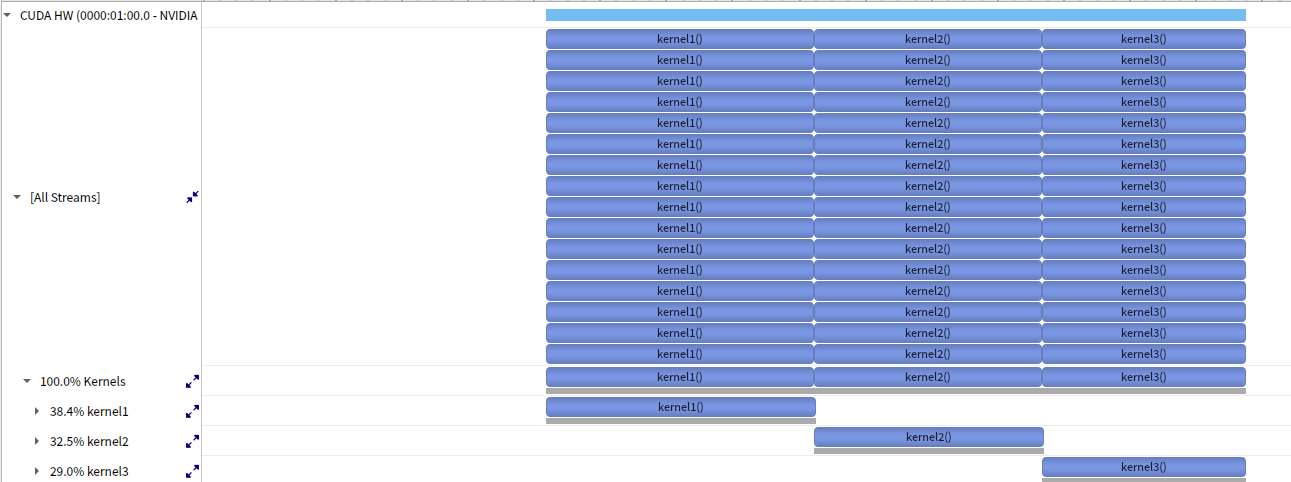
\includegraphics[width=0.9\textwidth]{assets/stream.png}
\subsubsection{分析总结}
\noindent
\begin{itemize}
	\item 利用流(stream)创建多个kernel的并发执行,实现grid level concurrency
	\item 在非默认流中launch kernel,需要在$kernel\_name<<<...>>>$第四个参数里面出入stream 标号
\end{itemize}


\subsection{kernel执行和数据传输重叠}
\subsubsection{实验结果}
\noindent
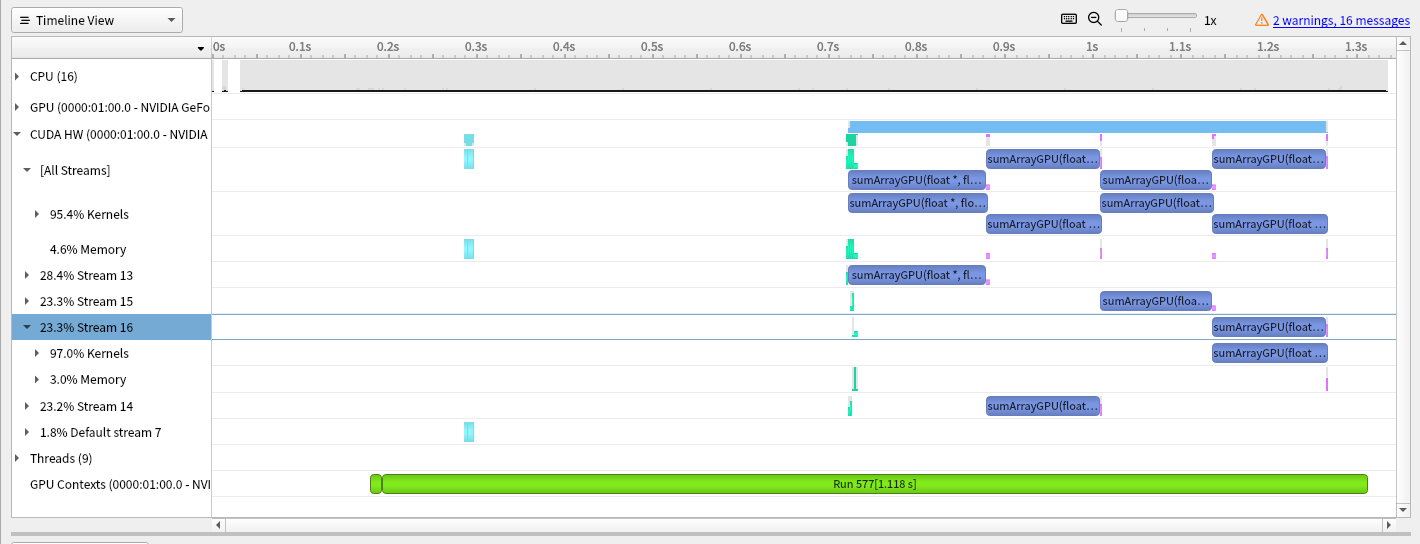
\includegraphics[width=0.9\textwidth]{assets/overlap.png}
\subsubsection{分析总结}
\noindent
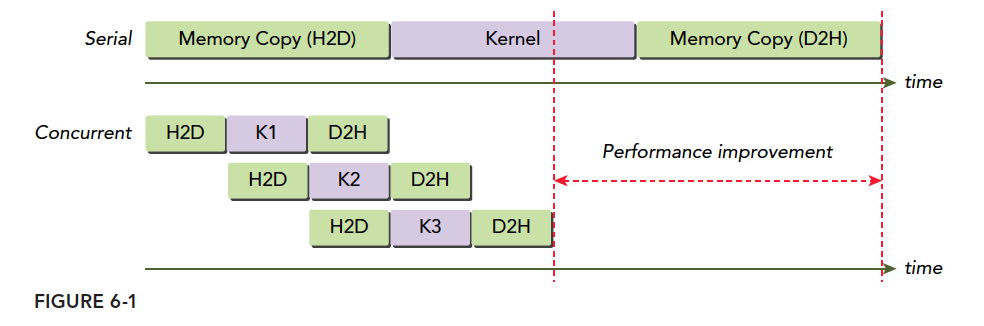
\includegraphics[width=0.9\textwidth]{assets/overlap2.png}
\begin{itemize}
	\item 不同流中内核相互重叠,内核执行和数据传输重叠,不同流中不同方向(HtoD or DtoH)的数据传输重叠
	\item 数据传输使用异步方式,注意异步处理的数据要声明称为固定内存
\end{itemize}

\section{总结}
\begin{itemize}
	\item 以熟悉cuda编程概念和跑通代码为主,未进行更好的调参或者性能优化
	\item 最开始性能测试命令ncu报错,未做更精细的性能分析(后重装cuda可以使用)
	\item 因为使用不同的GPU架构和CUDA版本,有些程序没有产生像书中分析那样的结果
	\item 还有更深入的优化并行算法的方法有待研究
\end{itemize}
\section{参考资料}
\noindent
1.《Professional CUDA C Programming》 
\end{document}